\documentclass[11pt]{article}
\setlength{\topmargin}{0in}
\setlength{\headheight}{0in}
\setlength{\headsep}{0in}
\setlength{\textheight}{8.7in}
\setlength{\textwidth}{6.5in}
\setlength{\oddsidemargin}{0in}
\setlength{\evensidemargin}{0in}
\setlength{\parindent}{0.3in}
\setlength{\parskip}{0.10in}

\special{papersize=8.5in,11in}
\setlength{\pdfpageheight}{\paperheight}
\setlength{\pdfpagewidth}{\paperwidth}

\usepackage{graphicx}
\usepackage{subfig}

\begin{document}

\title{Glacial cycles during the past three million years}
\author{Miles Wu}
\maketitle

\begin{abstract}
Ever since the formation of glaciers approximately three million years ago, the glaciers have waxed and waned in cycles. These cycles at first start with regular forty-one thousand year periods, but around one million years ago they become more erratic and violent. A paper by Huybers and another by Philander and Barreiro purporting to analyze and explain these cycles are reviewed, compared and contrasted.
\end{abstract}

\section{Introduction}
%how to measure ice volumes
The global ice volume can be inferred from looking at what is called the `$\delta^{18}$O' of sediment cores.
Deep sea sediment cores have foraminifera shells of calcium carbonate (chemical formula: CaCO$_3$).
Although oxygen most commonly has an atomic mass of $16$ ($99.8\%$), there is a less common but stable isotope with an atomic mass of $18$ ($0.2\%$) \cite{viu}.
In `$\delta^{18}$O' analysis we look at the ratio of these two stable isotopes in the carbonates in the sediment cores.
It has been found that during glacial periods the cores have a high $\delta^{18}$O' value.
As a result we can use these to infer the global ice volume as it is proportional to the $\delta^{18}$O' value.

%explain
This correlation between global ice volume and $\delta^{18}$O value can be explained.
The lighter $^{16}$O isotope moves slightly faster as it is lighter and therefore it evaporates slightly more frequently than the heavier isotope.
As a result water vapor is slightly $^{16}$O-enriched and it leaves the sea from which it evaporated slightly $^{18}$O-enriched.
The largest amount of evaporation takes place near the equator so it becomes heavier and this water vapor moves towards the poles where it rains and therefore the polar waters become lighter.
This Rayleigh fractionation becomes more pronounced the larger the global ice volume, as the ice at the polar regions store the lighter isotope from the polar seas \cite{viu}.

%so what are the phenomenon
Looking at these cores, geoscientists found that appearance of northern continental glaciers occurred at around three million years ago \cite{fedorov}.
This is thought to be well understood as just the conclusion of a longer gradual cooling trend \cite{huybers}.
However, after the onset of glaciation, the last three million years have had a dramatic increase in fluctuations, especially in ice volume.
This can be seen in Figure \ref{d18o}; the important thing to note is that the scale along the horizontal axis changes at $t=3~\textnormal{Ma}$ and therefore the fluctuations are significantly larger in amplitude.

% paper topic
The reason for the sudden onset of these severe glacial cycles and their patterns are a topic of present debate.
Huybers provides a plausible explanation for the timing of the cycles and does some statistical analysis to justify his explanation \cite{huybers}.
He further goes on and provides a simple model to describe the cycles.
Philander and Barreiro also propose a modification to Huybers' simple model.
In this paper we look at these two papers, comparing and contrasting their respective models.

\begin{figure}
  \centering
  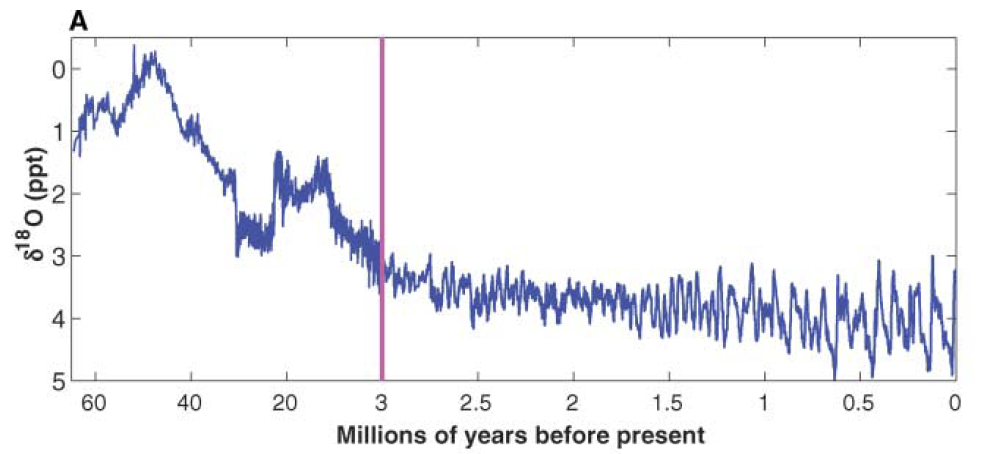
\includegraphics[width=4in]{d18o.png}
  \caption{The $\delta^{18}$O record from sediment cores, showing glacial ice volumes. Note the change in scale at three million years ago. Reproduced from \cite{huybers}.}
  \label{d18o}
\end{figure}

\section{Milankovitch Forcing}
%region definitions
In Figure \ref{d18o} there is another change around approximately $1.2~\textnormal{Ma}$, where the fluctuations in the global ice volume become even more abrupt and violent.
This change is known as the mid-Pleistocene transition.
We use this to split up the past three million years into two regions: the earlier calmer region from 3 Ma to 1.2 Ma and the later more violent region from 1.2 Ma to the present.
Let us examine the former region first.

%no disagreement about first part
Huybers, after analyzing these early pleistocene glacial cycles using Fourier transforms and spectral analysis, reports that these have a period of approximately forty thousand years \cite{huybers}.
Philander and Barreiro also report a similar thing, saying that there are oscillations with a period of forty-one thousand years \cite{philander}.
Both explain this through a phenomenon known as Milankovitch forcing, in particular the obliquity forcing, as this cycles in the phenomenon has a forty-one thousand year cycle; this seems a very reasonable explanation as it would be unlikely that it was a coincidence that they share the same period to within a small amount of uncertainty.

%what is Milankovitch forcing
Milankovitch forcing is the name given to climate forcing by the Earth's orbit.
There are three parameters of our orbit around the sun: eccentricity, obliquity and precession.
Eccentricity is a variable that relates the shape of the Earth's orbit relative to a circular orbit, obliquity is the tilt of the earth, and precession is the change in direction of the earth's rotation axis.
These three parameters are constantly changing and their cycles affect how much sunlight falls on the Earth and its glaciers, which in turn can influence glaciation or deglaciation rates through its warm rays.
Eccentricity has a one hundred thousand year period, precession a nineteen thousand and a twenty-three thousand year period and obliquity a forty-one thousand year period, so it makes a lot of sense to attribute the glacial cycles to obliquity cycles as it seems plausible that it could affect glacier rates \cite{uri}.

In the later region (1.2 Ma to the present) spectral analysis yields a different picture.
No longer is there a peak at forty thousand years, but instead there is a broad peak at one hundred thousand years \cite{huybers}; this change in cycle periods is a distinguishing feature of this second region compared to the first.
The cycles are actually either approximately eighty thousand years or one hundred thousand years and so the two peaks of the spectral analysis plot have just merged \cite{philander}.
Because the cycles are multiples of the obliquity cycle (forty thousand years) both Huyberr and Philander and Barreiro agree that the glaciation cycles are still controlled by the obliquity \cite{huybers}\cite{philander}.
There are other possible explanations stemming from eccentricity or precessions, but Huybers points out that eccentricity does not have a big enough effect to cause the glaciation cycles and precession forcing is anti-symmetric between the hemispheres but the glacial cycles are symmetric \cite{huybers}.
Attributing the cycles to obliquity seems reasonable and the reasons that Huybers puts forward for why it can't be other phenomenon seem plausible too.

%statistical test?
While it seems pretty conclusive for the first region (3 Ma to 1.2 Ma), it is not quite so obvious and clear-cut for the second region (1.2 Ma to the present); some kind of quantitative method is needed to justify the argument.
As a result, Huybers performs a statistical test as evidence for the validity of his explanation\cite{huybers}.
His formal hypothesis is that deglaciations are triggered at a specific point in the phase of the obliquity cycle, and conversely his null hypothesis is that they are independent of the phase of obliquity and therefore should be uniformly distributed with respect to obliquity phase.
Deglaciation events are identified from the $\delta^{18}$O record as large changes and thirty-six events are found: twenty from the first period and sixteen from the second.
The results from this statistical test are quite conclusive as Huybers finds that it is significant at the $99\%$ level for both the early and the late period.
This is also shown in a plot in Figure~\ref{hypotest}; the deglaciation events (red dot) are not uniformly distributed with respect to the obliquity phase (the large circle).

\begin{figure}
  \centering
  \subfloat[Early Pleistocene]{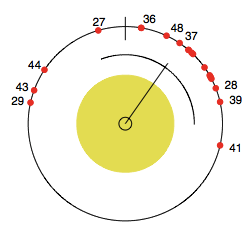
\includegraphics[width=2in]{hypotestc.png}}
  \subfloat[Late Pleistocene]{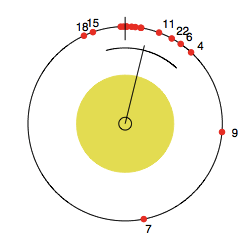
\includegraphics[width=2in]{hypotestd.png}}
  \caption{A diagram showing the obliquity phase at which each deglaciation occured for both the early and late Pleistocene periods. Each red dot is a deglaciation event, and the circle represents the phase angle of the obliquity. Reproduced from \cite{huybers}}
  \label{hypotest}
\end{figure}

%conclusion for this section
Obliquity cycles setting the pace for the glacial cycles is pretty convincing from the evidence presented by both Huybers and Philander and Barreiro.
Not only is it an explanation that makes sense and seems plausible, the statistical evidence from Huybers is very strong and is sufficient for us to conclude that obliquity is the root pacemaker for the glacial cycles.
Occam's razor is also another motivation for why obliquity cycles should be the cause of the glacial cycles in both the late and early Pleistocene.
This principle of science prefers the simpler explanation (less assumptions) for any given explanation of a phenomenon.
Here it is simpler that there is just one unified explanation and theory for glacial cycles that lasts throughout both periods, rather than two independent theories for each period, which would require another explanation for the transition too.

\section{Obliquity cycle skipping}
One mystery still remains: the glacial cycles in the late Pleistocene period do not match up with the obliquity cycles one-to-one and are some multiple of the forty-one thousand period.
Although we have shown that the deglaciation occurs at the same point in the obliquity cycle, we have not explained why it does not happen every cycle and usually one or two cycles are skipped in the late Pleistocene period.

%huybers model
Huybers offers a simple model to explain this phenomenon \cite{huybers}.
In this model, the global ice volume increases linearly with time until a threshold limit is reached.
When the threshold is reached an abrupt deglaciation occurs which resets the ice volume to the zero and it starts again.
The threshold also has a linear trend, but it also further has an additional term for obliquity.
Obliquity here is normalized to zero mean and has unit variance.
This model seems like it could reproduce the cycle skipping and the deglaciation occurring at a certain point in the obliquity phase, because the deglaciation threshold depends on the obliquity.
This makes it most likely that deglaciation occurs when obliquity is minimal (or maximal if the coefficient for the obliquity term is negative), which is what we found in the data.
The skipping occurs because it does not always reach the deglaciation threshold in one obliquity cycle.
At first it seems dubious that deglaciation would be so abrupt and severe, removing all glaciers over only a mere ten thousand years, but Huybers provides evidence for this, saying that various sophisticated ice-sheet models have simulated this behavior \cite{huybers}.

%comparison to data
Huybers claims that this simple model can reproduce the obliquity cycle skipping patterns that we see in the $\delta^{18}$O record in the last two million years to a large degree of accuracy \cite{huybers}.
However, it seems premature to attempt to use such a simple model to explain an extremely complex, non-linear and intricate system.
Although the model is plausibly justified, it is overly simplified (for example, constant linear growth and a guaranteed deglaciation to zero ice over exactly the same time every time) and could not possibly be expected to match the complex behavior of the data.
Given enough free parameters, any model can be made to match experimental data.
For example, a polynomial of degree $N$ can be made to go through $N$ points exactly with zero error, but this is a pointless exercise as it does not in any way imply that the polynomial is the correct equation.
Philander and Barriero agree with us on this, saying that ``the purpose of these models is not the realistic simulation of observations, but exploration of different modes of climate variability'' \cite{philander}.

%difference in model with philander
Philander and Barreiro propose a model similar to Huybers' but with a few differences \cite{philander}.
The growth of the ice volume is now more complicated: instead of just being a simple constant linear growth, it also has an exponential growth term, a term relating to the cube of the ice volume and a superimposed obliquity oscillation that increases in amplitude with ice volume.
These additional terms need to be justified or there is no point adding additional complication to a simpler model.
The exponential growth term is attributed to a feedback loop that accelerates the cooling.
The glaciers and their corresponding snow reflect sunlight, increasing the albedo and in turn lowering temperatures; the lowered temperatures then cause faster glaciation.
The superimposed amplifying obliquity oscillations are said to be because the obliquity affects the amount of sunlight melting the snow on the glaciers in summer, modifying the albedo.
The cubic term is attributed to a feedback associated with atmospheric carbon dioxide that only became significant around one million years ago.
On the other hand, the threshold is slightly simpler as is constant plus obliquity, rather than linear.
Once the threshold is reached the glaciers only ablate to one third of their previous size, not zero; this seems less extreme and more likely, though is still somewhat unjustified assumption.

%philander works too.
The model of Philander and Barreiro, in addition to the terms in the equation being justified by them, also seems a plausible candidate to explain the obliquity cycle skipping.
With the obliquity oscillations superimposed on the general glacial growth trend, it is more likely to reach the deglaciation threshold during a maximum (or minimum depending on the sign of the coefficient), which is what we need in our model as evidenced by the statistical test earlier.
One thing that we noticed was that the obliquity term in the threshold equation using the suggested parameter values in their paper has no effect.
Changing $\beta$ (default value $100$) to any value in the range of $0$ to $30000$ made absolutely no difference to a graph of ice volume for the past three millon years.
The reason for this is that the obliquity term (of the order of 100) is completely dwarfed by the constant term ($\alpha = 60000000$) and so it has no effect; this means that we can drop that term entirely as an easy simplification with no changes.
This simplification shows that in their model obliquity forcing only features in the growth equation and not the limiting threshold.

%parameters of philander
In many ways the model of Philander and Barreiro seems to be preferable and makes more sense than Huybers' model. Although the glacier growth equation is more complex, each term is justified and seems very plausible; both accelerating growth due to albedo feedback and a term dealing with obliquity are an obvious inclusion and one that surely have an effect on glacial growth.
The threshold equation being simpler is also a plus: Huybers' threshold has a linear trend with respect to time that has no justification, but Philander and Barreiro do away with this.

From playing around with the two models, it seems that the two models have one fundamentally different characteristic: the explanation behind the change from the early to late Pleistocene behavior (in early it does not skip any cycles, but in late it usually skips one or two).
In Huybers' model it arises because the threshold increases with time and so for the late time periods it takes longer to for the ice to grow and reach the threshold, taking more cycles.
This implies that in the future glacial cycles might take one hundred and sixty thousand years or even two hundred thousand years.
In the model of Philander and Barreiro, the change in cycle period occurs mainly because of the cubic carbon dioxide term coming into play.
Without that extremely rapid growth term it would take far too long for the ice to reach the threshold (based on their suggested parameters) and the cycles would be far too long.
Their model suggests that this carbon dioxide term coming into effect was the cause of the transition from early to late Pleistocene.
More research is warranted into the origin of this atmospheric carbon dioxide feedback and whether it can be such a huge growth term.
Perhaps more accurate dating can be done to determine if the carbon dioxide came into play at exactly the same time that the glaciation cycles changed or whether it was only around the time and not the root cause.

%chaotic
While recreating the graph of ice volume from Philander and Barreiro's paper (Figure 3), we investigated how subtle changes in the input parameters of the model would change the glacial cycles.
We found that even very tiny changes in the parameters caused huge changes, and past a certain point in the simulation it did not resemble the original graph at all.
To show this we plotted the ice volume from 1.5 million years ago to present based off the parameters listed in Philander and Barreiro's paper, and then overplotted another graph showing the ice volume but using a slightly modified parameter.
In Figure~\ref{alpha} we changed the constant term in the threshold equation (known as the maximum ice volume) by only a mere $1\%$.
At first there are no discernible differences, as expected for such a small change, but the behavior begins to diverge at six hundred thousand years ago.
Soon the behavior of the two curves are not alike at all and have become unrecognizable as once being near-identical.
This is known as the butterfly effect, named so because of the idea that a hurricane formation could depend on whether a butterfly had flapped its wings weeks prior.
This term refers to the very sensitive dependence on initial state and parameters in nonlinear chaotic systems.

\begin{figure}
  \centering
  % GNUPLOT: LaTeX picture with Postscript
\begingroup
  \makeatletter
  \providecommand\color[2][]{%
    \GenericError{(gnuplot) \space\space\space\@spaces}{%
      Package color not loaded in conjunction with
      terminal option `colourtext'%
    }{See the gnuplot documentation for explanation.%
    }{Either use 'blacktext' in gnuplot or load the package
      color.sty in LaTeX.}%
    \renewcommand\color[2][]{}%
  }%
  \providecommand\includegraphics[2][]{%
    \GenericError{(gnuplot) \space\space\space\@spaces}{%
      Package graphicx or graphics not loaded%
    }{See the gnuplot documentation for explanation.%
    }{The gnuplot epslatex terminal needs graphicx.sty or graphics.sty.}%
    \renewcommand\includegraphics[2][]{}%
  }%
  \providecommand\rotatebox[2]{#2}%
  \@ifundefined{ifGPcolor}{%
    \newif\ifGPcolor
    \GPcolortrue
  }{}%
  \@ifundefined{ifGPblacktext}{%
    \newif\ifGPblacktext
    \GPblacktexttrue
  }{}%
  % define a \g@addto@macro without @ in the name:
  \let\gplgaddtomacro\g@addto@macro
  % define empty templates for all commands taking text:
  \gdef\gplbacktext{}%
  \gdef\gplfronttext{}%
  \makeatother
  \ifGPblacktext
    % no textcolor at all
    \def\colorrgb#1{}%
    \def\colorgray#1{}%
  \else
    % gray or color?
    \ifGPcolor
      \def\colorrgb#1{\color[rgb]{#1}}%
      \def\colorgray#1{\color[gray]{#1}}%
      \expandafter\def\csname LTw\endcsname{\color{white}}%
      \expandafter\def\csname LTb\endcsname{\color{black}}%
      \expandafter\def\csname LTa\endcsname{\color{black}}%
      \expandafter\def\csname LT0\endcsname{\color[rgb]{1,0,0}}%
      \expandafter\def\csname LT1\endcsname{\color[rgb]{0,1,0}}%
      \expandafter\def\csname LT2\endcsname{\color[rgb]{0,0,1}}%
      \expandafter\def\csname LT3\endcsname{\color[rgb]{1,0,1}}%
      \expandafter\def\csname LT4\endcsname{\color[rgb]{0,1,1}}%
      \expandafter\def\csname LT5\endcsname{\color[rgb]{1,1,0}}%
      \expandafter\def\csname LT6\endcsname{\color[rgb]{0,0,0}}%
      \expandafter\def\csname LT7\endcsname{\color[rgb]{1,0.3,0}}%
      \expandafter\def\csname LT8\endcsname{\color[rgb]{0.5,0.5,0.5}}%
    \else
      % gray
      \def\colorrgb#1{\color{black}}%
      \def\colorgray#1{\color[gray]{#1}}%
      \expandafter\def\csname LTw\endcsname{\color{white}}%
      \expandafter\def\csname LTb\endcsname{\color{black}}%
      \expandafter\def\csname LTa\endcsname{\color{black}}%
      \expandafter\def\csname LT0\endcsname{\color{black}}%
      \expandafter\def\csname LT1\endcsname{\color{black}}%
      \expandafter\def\csname LT2\endcsname{\color{black}}%
      \expandafter\def\csname LT3\endcsname{\color{black}}%
      \expandafter\def\csname LT4\endcsname{\color{black}}%
      \expandafter\def\csname LT5\endcsname{\color{black}}%
      \expandafter\def\csname LT6\endcsname{\color{black}}%
      \expandafter\def\csname LT7\endcsname{\color{black}}%
      \expandafter\def\csname LT8\endcsname{\color{black}}%
    \fi
  \fi
  \setlength{\unitlength}{0.0500bp}%
  \begin{picture}(9000.00,6720.00)%
    \gplgaddtomacro\gplbacktext{%
      \csname LTb\endcsname%
      \put(1210,704){\makebox(0,0)[r]{\strut{} 0}}%
      \put(1210,1526){\makebox(0,0)[r]{\strut{} 1e+07}}%
      \put(1210,2347){\makebox(0,0)[r]{\strut{} 2e+07}}%
      \put(1210,3169){\makebox(0,0)[r]{\strut{} 3e+07}}%
      \put(1210,3990){\makebox(0,0)[r]{\strut{} 4e+07}}%
      \put(1210,4812){\makebox(0,0)[r]{\strut{} 5e+07}}%
      \put(1210,5633){\makebox(0,0)[r]{\strut{} 6e+07}}%
      \put(1210,6455){\makebox(0,0)[r]{\strut{} 7e+07}}%
      \put(1342,484){\makebox(0,0){\strut{}-3000}}%
      \put(2552,484){\makebox(0,0){\strut{}-2500}}%
      \put(3762,484){\makebox(0,0){\strut{}-2000}}%
      \put(4972,484){\makebox(0,0){\strut{}-1500}}%
      \put(6182,484){\makebox(0,0){\strut{}-1000}}%
      \put(7392,484){\makebox(0,0){\strut{}-500}}%
      \put(8602,484){\makebox(0,0){\strut{} 0}}%
      \put(176,3579){\rotatebox{-270}{\makebox(0,0){\strut{}Ice volume}}}%
      \put(4972,154){\makebox(0,0){\strut{}Time before Present /Kyr}}%
    }%
    \gplgaddtomacro\gplfronttext{%
      \csname LTb\endcsname%
      \put(7615,6282){\makebox(0,0)[r]{\strut{}$\alpha = 6.00 \times 10^7$}}%
      \csname LTb\endcsname%
      \put(7615,6062){\makebox(0,0)[r]{\strut{}$\alpha = 5.94 \times 10^7$}}%
    }%
    \gplbacktext
    \put(0,0){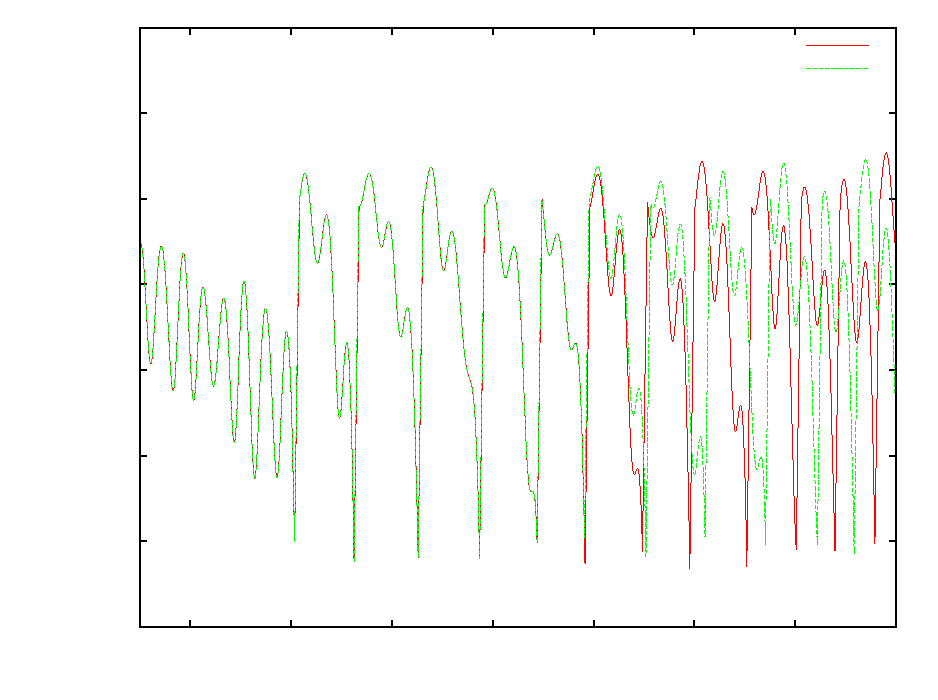
\includegraphics{alpha}}%
    \gplfronttext
  \end{picture}%
\endgroup

  \caption{Glacial ice volumes for the past one and half million years simulated from the Philander and Barreiro model. Two simulations were made with slightly different input parameters (by one percent).}
  \label{alpha}
\end{figure}

The chaos in this system can make it hard to analyze, especially in terms of observing the patterns.
Attempting to perform long time duration simulations to accurately simulate or fit to data will be impossible.
This is much the same as weather predictions, which can only offer short range forecasts to any degree of useful accuracy.
This is not saying that the Philander and Barreiro model is wrong; quite the opposite, it seems perfectly possible that glaciation is chaotic just like the weather.
Although we did not test it, the Huybers model probably does not suffer from the same problem, because after each cycle the ice volume resets to zero; this gives it plenty of opportunities to reconverge after diverging.
As a result it might be preferred to use this model as it is more analyzable until there is stronger evidence for chaotic behavior.


\section{Conclusion}
There are very strong indications that obliquity is the pacemaker for these glacial cycles in both the early and the late Pleistocene periods.
Not only does it make sense qualitatively, the statistical test that Huybers performs also provides solid evidence for it.

While both papers provide physically reasonable models to explain obliquity cycle skipping, neither are conclusively correct nor is it obvious which is better.
Although there are some difference between them, in particular in explaining the transition from early to the late period, both tie the cycles into reaching a threshold for sudden deglaciation at varying periods because of obliquity forcing (this also maintains the deglaciation's dependence on the phase of obliquity as determined by the statistical test).
More research is needed, perhaps into the carbon dioxide cubic term, in order to determine which is the more accurate model.

\begin{thebibliography}{9}
	\bibitem{huybers}
		Huybers, P. Glacial variability over the last two million years: an extended depth-derived agemodel, continuous obliquity pacing, and the Pleistocene progression. \emph{Quaternary Science Reviews} 26: 37--55 (2007)
	\bibitem{fedorov}
		Fedorov, A \emph{et al}. The Pliocene Paradox (Mechanisms for a Permanent El Nino). \emph{Science} 312: 1485 (2006)
    \bibitem{philander}
        Philander, S and Barreiro, M. A Tropical Perspective on The Increase in Climate Sensitivity Over the Past 3 Million Years. (2011 Preprint)
	\bibitem{viu}
		Earle, S. Oxygen Isotope fractionation \emph{http://web.viu.ca/earle/\\geol-412/oxygen\%20Isotope\%20fractionation.pdf}
    \bibitem{uri}
        Rutherford, S. Milankovich Cycles in Paleoclimate. \emph{http://deschutes.gso.uri.edu/\\~rutherfo/milankovitch.html}
\end{thebibliography}

\end{document} 